\section{Dependence}

Recall that in \eqref{eq:cond_ind} we assumed conditionally independent observations
given the object (namely, its position and class):
%
\begin{align}
  p( \mathbf{Z} | obj_c ) &= \prod_{i=1}^{n} { p( z_i | obj_c) }
  \text{.}
\end{align}
%
However, this is not the case. Consider intraclass variation of objects. A star
object might not always have the same size. In this case, one observation might
capture some of this variation, and thus be informative for the next
observation. For example, if a LIDAR observation is closer to use, that might
indicate that the object is on the large size, and thus the next observation is
likely to be close as well.

Ideally, we would capture the full distribution $p ( \mathbf{Z} | obj_c )$. However,
this is not tractable. We find that making the conditionally independent
assumption hinders the quality of multiclass detection, as it is easy to confuse
different classes. We compromise by creating a "2-gram" model:
%
\begin{align}
  p( \mathbf{Z} | obj_c ) &= \left( \prod_{i=2}^{n} { p( z_i | obj_c, z_{i-1}) }
  \right) p( z_1 | obj_c)
  \text{,}
\end{align}
%
where each observation depends only on the one directly preceding it (note that
with this terminology, we refer to the previous model as the "1-gram" model).
Generally speaking, we can construct this sort of $n$-gram model for any $n$,
but as $n$ grows the distribution quickly becomes more challenging to capture
with simulated training data.

\begin{figure*}
  \centering
  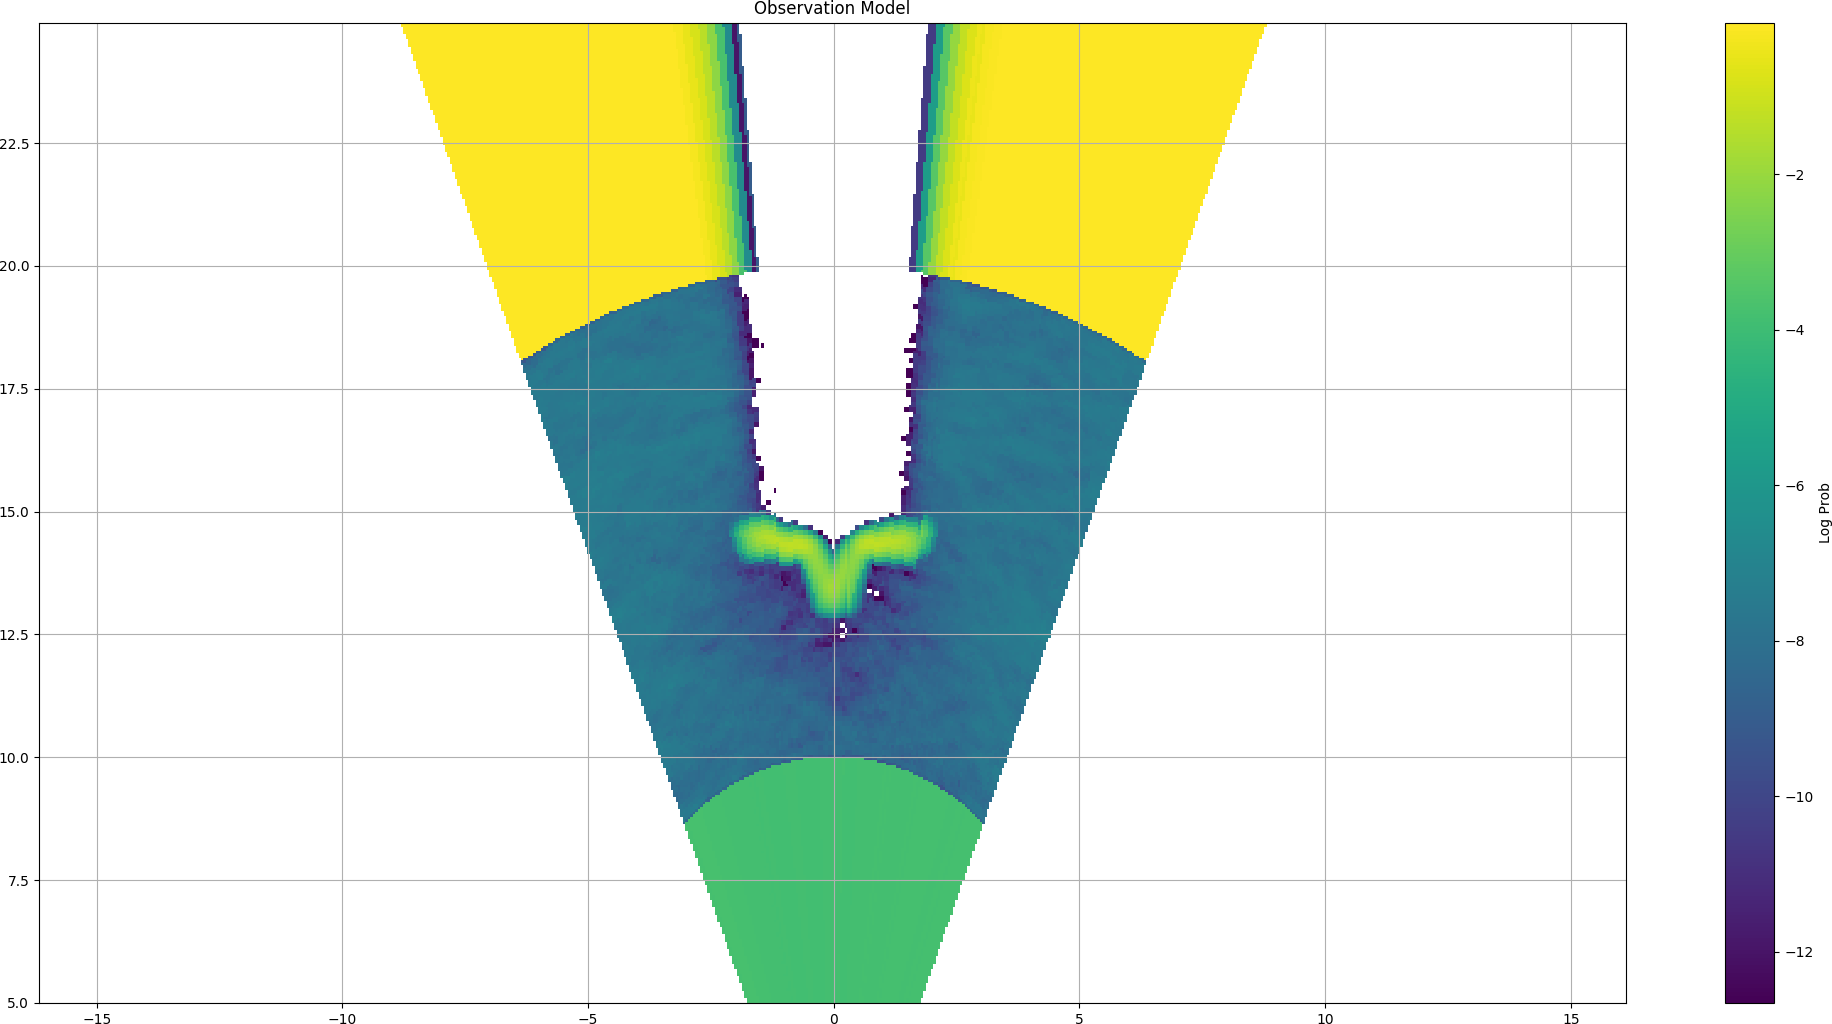
\includegraphics[width=\textwidth]{figures/star_model.png}
  \caption{Simulation. On the left is the simular LIDAR scan of the environment.
    The right figure depicts the ground truth position of all objects in the
    scene.}
  \label{fig:star_model}
\end{figure*}

\begin{figure*}
  \centering
  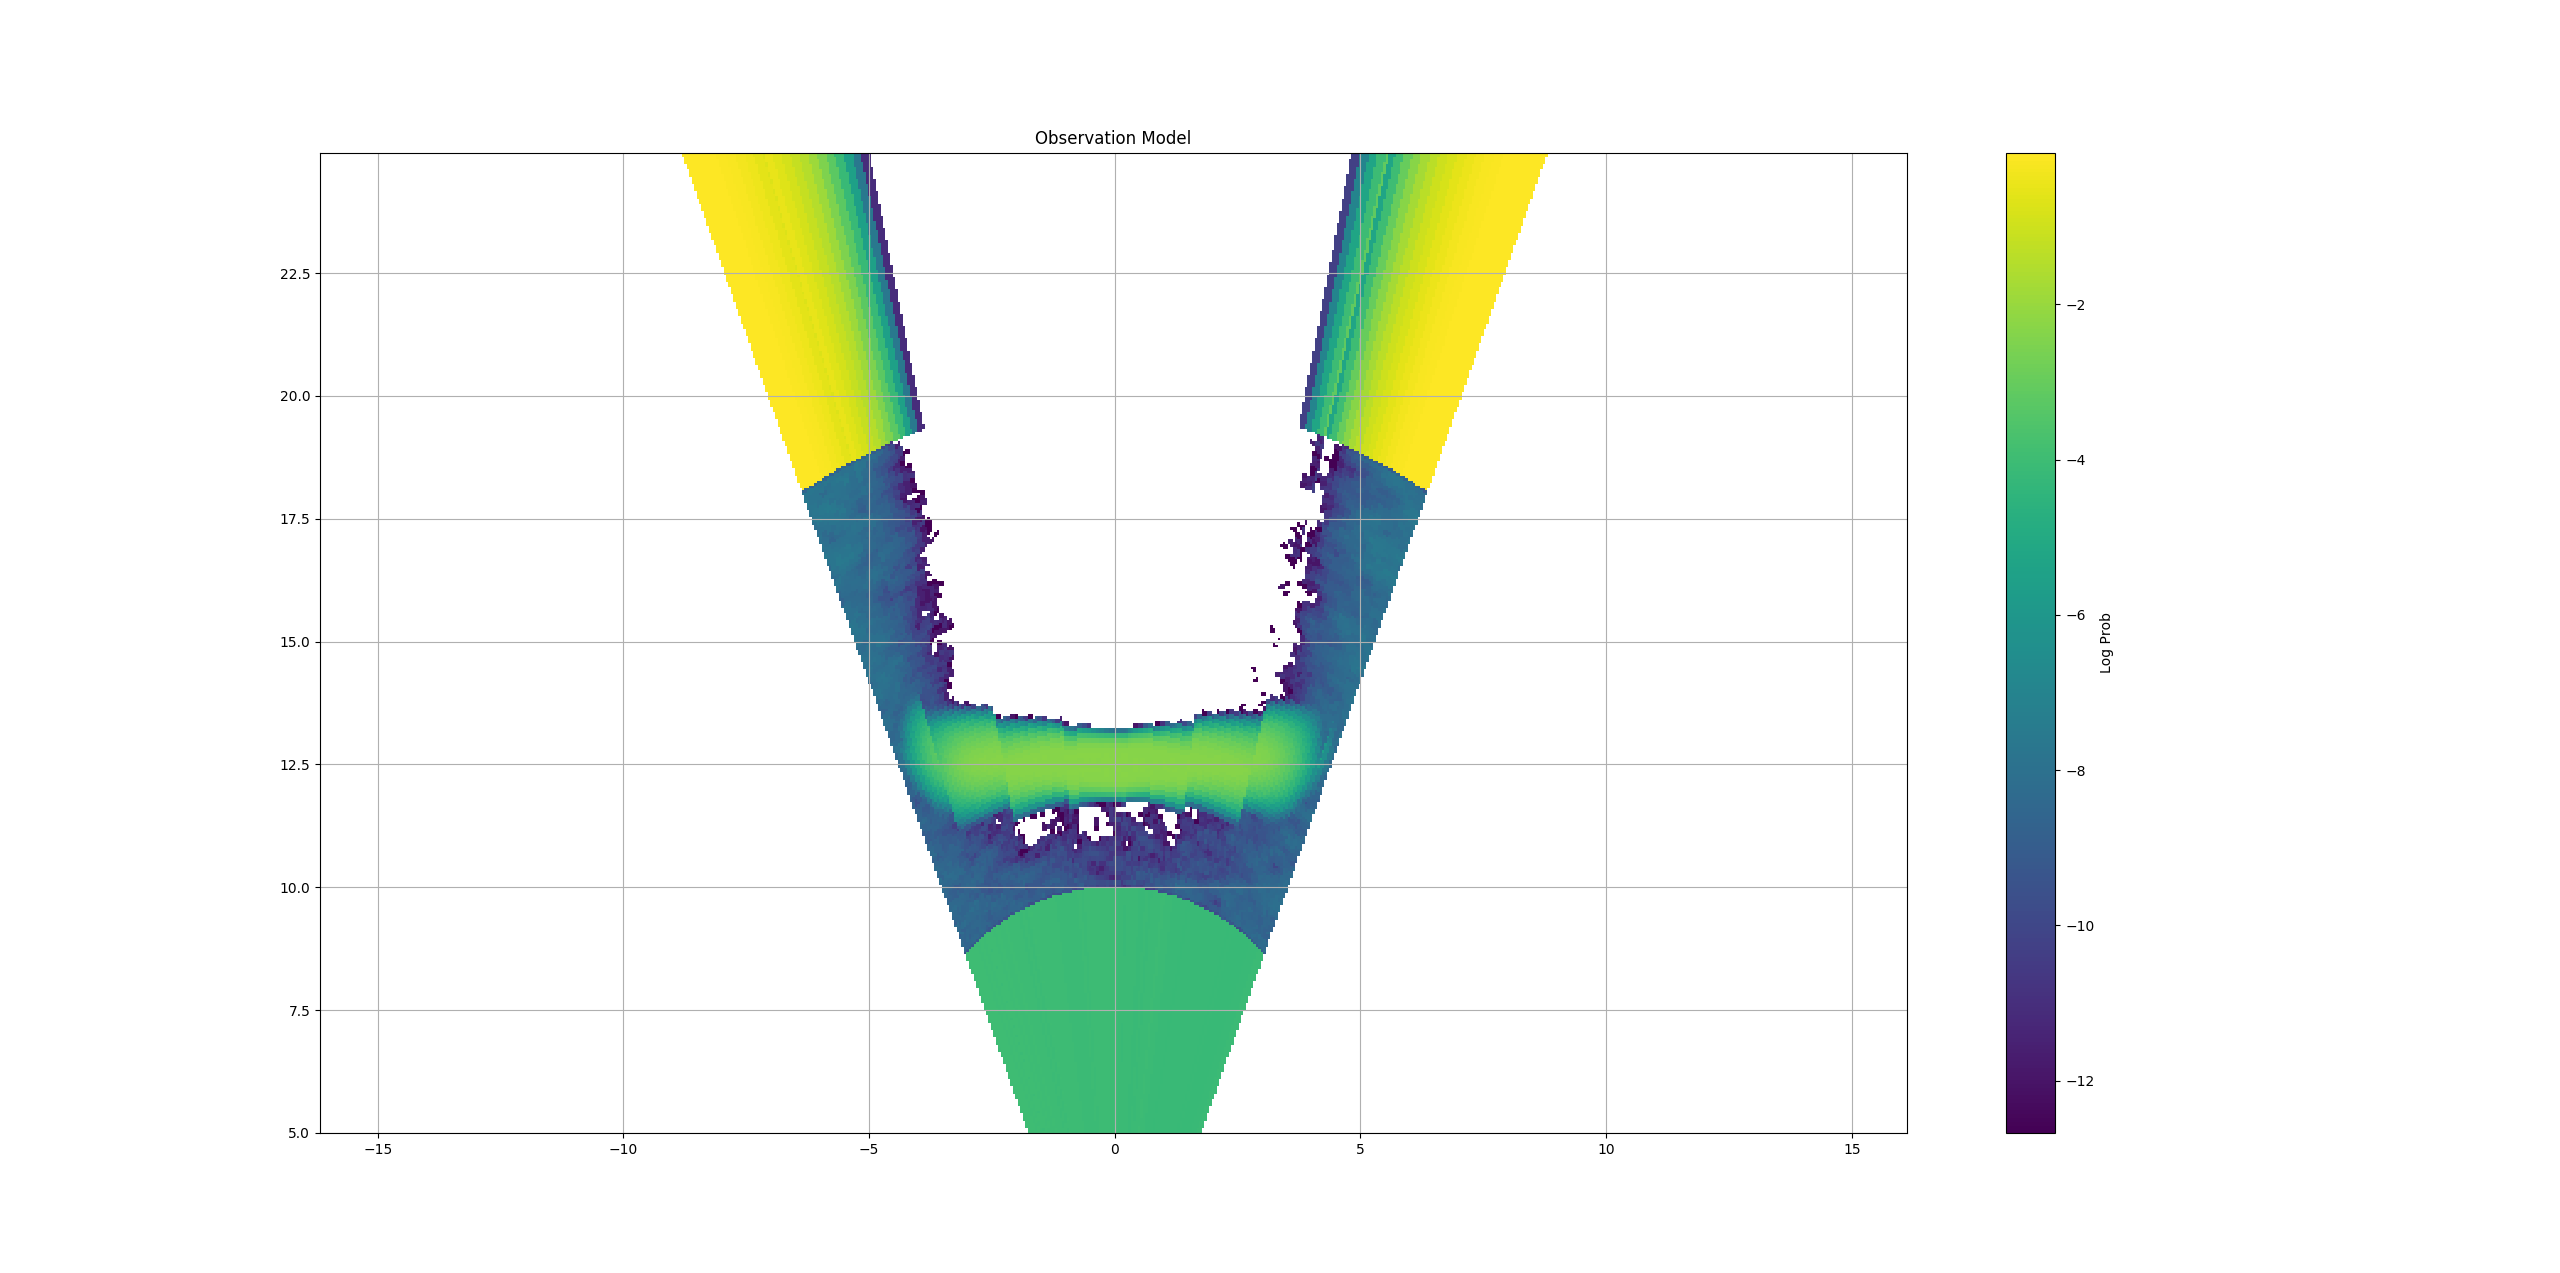
\includegraphics[width=\textwidth]{figures/box_model.png}
  \caption{Simulation. On the left is the simular LIDAR scan of the environment.
    The right figure depicts the ground truth position of all objects in the
    scene.}
  \label{fig:box_model}
\end{figure*}
